
\chapter{Jobmanager}


\section{Einleitung}
\begin{figure}
	\centering
	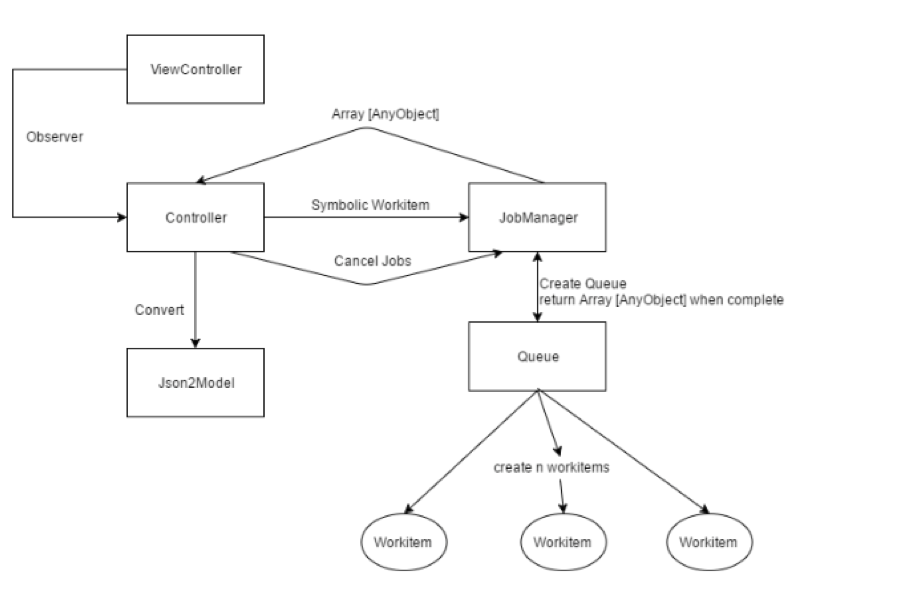
\includegraphics[scale=0.6]{JobManager-Architektur.png}
	\caption{Architektur und Integration des JobManagers in die Stundenplan App}
	\label{img:JobManager-Architektur}
\end{figure}
Im folgenden Dokument, wird auf die Funktionsweise des JobManagers in der iOS Stundenplan App der Hochschule Hof näher eingegangen.
\newline Innerhalb der Applikation verwaltet der JobManager alle Jobanfragen und delegiert die Aufgaben asynchron an die jeweils unterliegende Schicht.
\newline
\newline Jede Instanz des JobMangers verwaltet seine eigene Warteschlange (Queue). In dieser Warteschlange können sich n Workitems befinden. Jedes Workitem stellt eine Netzwerkanfrage (einen Job) dar. Ergebnisse werden in der Warteschlange gesammelt und sobald alle Ergebnisse vorliegen, werden diese an den Auftraggeber weitergegeben.
\newline
Eine Abbruchfunktion für noch offene Jobs lässt den Vorgang jederzeit unterbrechen.
\newpage
\section{Ablauf}
Der Ablauf des JobManagers und die Verwendung für den Benutzer lässt sich in folgende Unterpunkte unterteilen:
\newline
\subsection{Erstellen des JobManagers}
Der JobManager wird ohne speziellen Konstruktor erstellt. Dazu reicht ein 
\newline  \textit{var myJobManager : JobManager = JobManager()}.

\subsection{Observer anmelden}
Ebenso ist das Anmelden des Observers schnell erledigt. Hierzu muss der jeweilige Controller lediglich das \textit{DataObserverProtocol}  implementieren und mittels
\newline
\newline
\textit{self.myJobManager.addNewObserver(o: self)}
\newline
\newline sich beim JobManager als Observer anmelden.

\subsection{Anfrage}
Wurde der JobManager erstellt und man hat sich als Observer angemeldet, so kann man eine neue Jobanfrage an den JobManager stellen. Eine Anfrage könnte so aussehen:
\newline
\newline \textit{myJobManager.NetworkJob(url: urlString, username: myUsername, password: myPassword)}
\newline
\newline Hier ist zu beachten, dass das einfügen eines Usernames und eines Passwortes optionale Parameter sind. 

\subsection{Ergebnis}
Sind alle Jobs erfolgreich beendet worden, so sendet der JobManager die Daten als \textit{AnyObject} an die update(o: AnyObject) Methode des Oberservers. 
\newline
\subsection{Aktuelle Version}
In der aktuellen Version ist es möglich den JobManger mehrmals zu verwenden. Eine neue Instanziierung ist nicht notwendig, wird jedoch für einen sauberen Ablauf empfohlen.



